\chapter{Introduzione al calcolo numerico}

Grazie al costante sviluppo dei computers negli scorsi decenni, la comunità scientifica ha avuto modo di usufruire di strumenti di calcolo sempre più precisi e complessi, necessari per risolvere alcuni problemi di vario tipo. Questo sviluppo ha visto anche un cospicuo interesse verso i metodi di calcolo numerico, che permettono di risolvere in modo non-analitico problemi specifici che non sarebbero, altrimenti, risolvibili. Infatti, seppur non esista sempre una soluzione analitica, \textbf{esiste sempre una soluzione numerica} per un modello matematico \textbf{ben posto} e \textbf{condizionato}, che assuma tuttavia certe assunzioni del corrispondente modello fisico.
\nl
La realtà infatti non è sempre modellabile attraverso semplici formule fisiche: a volte ci sono parecchie variabili da tenere in conto quando si cerca di risolvere un problema, e non è sempre plausibile considerare tutte queste variabili assieme, soprattutto se il problema va risolto senza l'assistenza di un calcolatore. Consideriamo il seguente esempio: un giocatore di golf colpisce una pallina con una certa velocità $U$, e noi vogliamo sapere per quale angolo $\alpha$ la distanza che verrebbe percorsa dalla pallina da golf sarebbe massima prima che quest'ultima tocchi terra.
\nl
Grazie alla seconda legge di Newton, possiamo calcolare la distanza percorsa dalla pallina, e se trascurassimo la resistenza dell'aria sarebbe abbastanza semplice trovare la soluzione analitica. Tuttavia, considerando questa resistenza, le equazioni del moto si complicano notevolmente, e determinare la soluzione analitica diventa ora impossibile. Tuttavia, la soluzione numerica rimane calcolabile attraverso l'impiego di metodi numerici adatti.
\nl
È comunque importante considerare anche il tipo di modello utilizzato: in base al modello matematico di partenza e al metodo utilizzato, si possono ottenere risultati diversi. L'importante è saper scegliere il metodo giusto e l'approssimazione migliore del modello.
\nl
Per il calcolo numerico, la risoluzione di un problema avviene attraverso i seguenti steps:
\begin{itemize}
    \item formulare un \textbf{modello matematico} in base al problema dato, che diventi uno schema per definire il metodo numerico e l'algoritmo di soluzione;
    \item scegliere un \textbf{metodo numerico} che aiuti nella risoluzione del problema;
    \item definire un \textbf{algoritmo} che porti alla soluzione desiderata;
    \item analizzare la \textbf{soluzione numerica} e interpretarla, capendo se quest'ultima sia una valida soluzione o meno. Si dice che una soluzione numerica sia \textbf{accettabile} se e solo se sia possibile \textbf{stimare gli errori} che accompagnano la soluzione stessa.
\end{itemize}

\section{Errori di approssimazione}

Quando si calcola una soluzione numerica, ci sono varie, possibili fonti di errori che possono condizionare il risultato finale. È possibile avere errori di \textbf{misura} (dati dalla precisione dello strumento), \textbf{inerenti} (creati da un'eccessiva semplificazione del modello reale), di \textbf{troncamento} (generati da una discretizzazione del risultato, generalmente presenti quando si usano metodi numerici che richiedono convergenza), e di \textbf{arrotondamento} (creati dalla macchina che performa i calcoli, in quando la precisione è sempre limitata).
\nl
Ogni computer dispone di un sistema numerico piuttosto primitivo: questo infatti dispone di un sistema \textbf{finito} di numeri, la cui lunghezza è anch'essa \textbf{finita}. Se normalmente, in campi analitici, siamo abituati a pensare con un insieme di numeri infinito (come quello dei numeri reali, $\mathbb{R}$), con i computer, quando si performano calcoli di analisi numerica, si considera un insieme ristretto, detto dei \textbf{numeri macchina} $\mathbb{F}$. Consideriamo ad esempio alcune delle costanti più famose nel mondo matematico: $\pi$, $e$ e $\sqrt{2}$. Noi sappiamo che questi numeri sono irrazionali, e che si espandono all'infinito. Proviamo a chiedere a una macchina di dirci quali sono questi numeri. Eseguendo il seguente script di Python, otterremo il seguente risultato:

\begin{codeblock}{Rounding.py}
    \begin{lstlisting}[language = Python]
import numpy as np
from math import sqrt

print(np.pi, np.e, sqrt(2), sep="\n")\end{lstlisting}
    \vspace{11pt}
    \begin{tcolorbox}[colback = black!95!Periwinkle!90]
        \begin{lstlisting}[style = notexterm]
Out[1]: 3.141592653589793
        2.718281828459045
        1.4142135623730951\end{lstlisting}
    \end{tcolorbox}
\end{codeblock}

Noi sappiamo che in realtà questi numeri si estendono molto più in profondità di quello che ci ha ritornato Python. Infatti:
\begin{itemize}
    \item $\pi = 3,1415926535897932384626433...$;
    \item $e = 2,71828182845904523536...$;
    \item $\sqrt{2} = 1,4142135623730950488...$
\end{itemize}

Qua notiamo già uno dei primi errori che si incontra quando si usa un calcolatore: i numeri sono \textbf{arrotondati} ad una certa cifra. L'arrotondamento genera spesso qualche tipo di errore, ma è necessario che i numeri subiscano una procedura di arrotondamento prima di poter essere usati da un calcolatore, poiché altrimenti non entrerebbero nella memoria di quest'ultimo, che ricordiamo essere limitata.

\begin{definition}{Errore di arrotondamento}
    Definitiamo l'\textbf{errore di arrotondamento} come la \textbf{differenza} tra il \textbf{numero reale} $x \in \mathbb{R}$ e il \textbf{numero macchina} $m \in \mathbb{F}$ corrispondente:
    \[ e_\text{arr} = x - m \]
\end{definition}

Se un calcolatore approssima tutti i numeri alla $D$esima cifra decimale, allora diciamo che l'errore di arrotondamento è compreso nell'\textbf{intervallo} $[-0,5 \cdot 10^{-D}, \; +0,5 \cdot 10^{-D}]$.
\nl
Riguardo lo scopo di queste note: MATLAB verrà usato durante il corso per implementare certi metodi numerici. Tale linguaggio di programmazione lavora con 15 cifre decimali significative. Fino a quando non verrà introdotto MATLAB tuttavia, verrà usato Python, che ne usa fino a 17 (anche se negli esempi precedenti $\pi$ e $e$ hanno usato solo 15 cifre, probabilmente a causa del pacchetto \verb|numpy|).
\nl
Consideriamo un esempio per comprendere l'importanza degli errori di arrotondamento:
\begin{example}
    Si considerino le due funzioni seguenti, che sono algebricamente equivalenti:
    \[ q_1(x) \eq (x - 1)^7 \quad \quad q_2(x) \eq x^7 - 7x^6 + 21x^5 - 35x^4 + 35x^3 - 21x^2 + 7x - 1 \]

    Vogliamo calcolare il valore numerico di $q_1(x)$ e $q_2(x)$ con due valori di $x$, ovverosia $1$ e $1,0001$, e confrontare il loro valore esatto con l'errore di arrotondamento. Vogliamo inoltre usare una macchina che lavori con 15 cifre significative. Usando il seguente script in Python, possiamo ottenere i nostri risultati:
    \begin{codeblock}{ApproxExample.py}
        \begin{lstlisting}[language = Python]
from math import pow

def q1(x) -> float:
    return (x - 1) ** 7

def q2(x) -> float:
    return pow(x, 7) - 7 * pow(x, 6) + 21 * pow(x, 5) \
        - 35 * pow(x, 4) + 35 * pow(x, 3) - 21 * pow(x, 2) + 7 * x - 1

def rounding_error(real, machine) -> float:
    return float(real) - float(machine)

# La lista contiene tuple del tipo (x, valore_reale)
for i, expect in [(1, 0), (1.0001, 10**(-28))]:
    # Approssimazione del numero alla 10a cifra decimale
    res1, res2 = "{0:.10g}".format(q1(i)), "{0:.10g}".format(q2(i))
    err1, err2 = rounding_error(expect, res1), rounding_error(expect, res2)
    print(f"With x = {i}, expect {expect}\nQ1 = {res1} | E1 = {err1}\nQ2 = {res2} | E2 = {err2}\n")\end{lstlisting}
        \nl
        \begin{tcolorbox}[colback = black!95!Periwinkle!90]
            \begin{lstlisting}[style = notexterm]
Out[1]: With x = 1, expect 0
        Q1 = 0 | E1 = 0.0
        Q2 = 0 | E2 = 0.0

        With x = 1.0001, expect 1e-28
        Q1 = 1e-28 | E1 = 0.0
        Q2 = 1.776356839e-15 | E2 = -1.7763568389999e-15\end{lstlisting}
        \end{tcolorbox}
    \end{codeblock}

    Come possiamo notare dall'output dello script, con $x = 1$ non c'è alcuna differenza tra $q_1(x)$ e $q_2(x)$, ma con $x = 1,0001$ iniziano ad esserci le prime differenze. Infatti, nel secondo caso abbiamo un errore di arrotondamento di circa $-1,78 \cdot 10^{-15}$. Questo semplice esempio dimostra come due quantità che sono algebricamente uguali possono in realtà portare a due risultati numerici completamente diversi.
    \nl
    Questo comportamento può essere inoltre osservato attraverso il seguente grafico:
    \begin{center}
        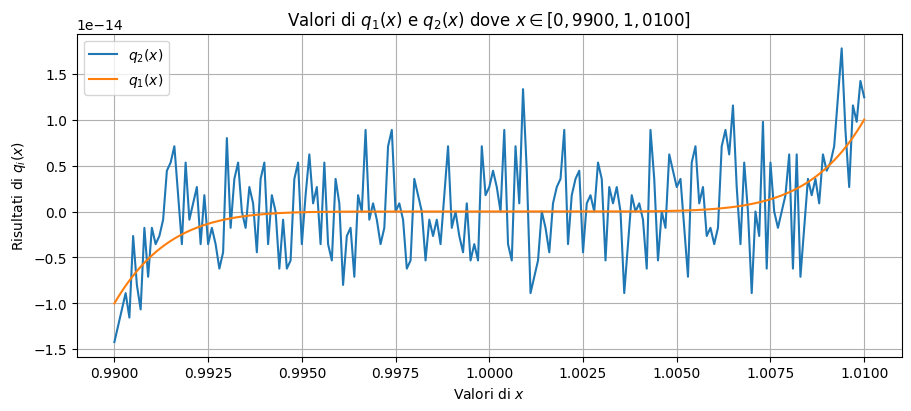
\includegraphics[width = \linewidth]{assets/image-001.png}
    \end{center}

    Notiamo infatti che, mentre $q_1(x)$ ha un comportamento più lineare, $q_2(x)$ è molto più scabro, e questo accade proprio a causa degli errori di approssimazione.
\end{example}

\section{La Rappresentazione IEEE 754}

Ogni numero reale $x$ può essere espresso come una sequenza di infinite cifre, e tale sequenza dipende dalla \textbf{base di rappresentazione} $\beta$. Di norma, la base con cui noi esseri umani facciamo calcoli è $\beta = 10$.
\nl
Qualsiasi cifra può essere espressa in qualsiasi base. Per farlo, faremo un esempio con $\pi$. Il numero infatti può essere scritto come segue:
\[ \pi \eq 3,14159... \eq \frac{3}{10^0} + \frac{1}{10^{-1}} + \frac{4}{10^{-2}} + \frac{1}{10^{-3}} + \frac{5}{10^{-4}} + \frac{9}{10^{-5}} + ... \]

L'idea è che per esprimere un qualsiasi numero $x$ in una base $\beta$, possiamo scrivere il numero come
\[ x \eq x_m \cdot \beta^m + x_{m-1} \cdot \beta^{m-1} + ... + x_{1} \cdot \beta^{1} + x_{0} \cdot \beta^{0} + x_{-1} \cdot \beta^{-1} + ... + x_{-m} \cdot \beta^{-m} \]

dove $0 \leq x_i \leq \beta - 1, \; \forall \; i \in [m, \; -m]$.
\nl
Sappiamo che i computer funzionano in codice binario, quindi non possono interpretare i numeri in base decimale come facciamo noi umani. Per poter far sì che un computer riconosca un numero, questo va prima convertito in base 2. Ci sono vari modi per rappresentare un numero in binario: che sia con o senza segno, a virgola mobile o meno... C'è tuttavia uno standard che i computer adottano, che è stato sviluppato dall'IEEE, che viene usato per rappresentare tutti i numeri in binario, che abbiano un segno o che siano a virgola mobile: l'\textbf{IEEE 754}.
\nl
Per questo standard, ogni numero può essere espresso nella seguente rappresentazione:
\[ x \eq \underbrace{\pm}_{\text{Segno}} \underbrace{(1 + a_{-1} \cdot 2^{-1} + a_{-2} \cdot 2^{-2} + a_{-3} \cdot 2^{-3} + ... + a_{-m} \cdot 2^{-m})}_{\text{Mantissa normalizzata}} \cdot \underbrace{2^e}_{\text{Esponente}} \]
\begin{center}
    \begin{tabular}{|c||c||c|}
        \hline
        $s$ & \hspace{1cm}$e$\hspace{1cm} & \hspace{3cm}$m$\hspace{3cm} \\
        \hline
    \end{tabular}
\end{center}

dove il segno viene rappresentato con 1 bit, la mantissa con $m$ bits e l'esponente con $n$ bits. Generalmente i numeri in IEEE 754 si possono esprimere con 16 (precisione dimezzata), 32 (singola precisione) o 64 bits (precisione doppia). Segue una tabella che segna quanti bits vengono assegnati ad ogni formato:
\begin{center}
    \begin{tabular}{|c|c|c|c|c|c|}
        \hline
        \textbf{Formato} & \textbf{Segno} & \textbf{Esponente} & \textbf{Mantissa} & \textbf{Bias} & \makecell{\textbf{Numero totale}\\\textbf{di bits}} \\
        \hline\hline
        \textbf{Precisione mezza} & 1 & 5 & 10 & 15 & 16 \\
        \hline
        \textbf{Singola precisione} & 1 & 8 & 23 & 127 & 32 \\
        \hline
        \textbf{Doppia precisione} & 1 & 11 & 52 & 1023 & 64 \\
        \hline
    \end{tabular}
\end{center}

Dato che i computer hanno una precisione finita, limitata a $p$ cifre, è chiaramente impossibile per questi rappresentare numeri che abbiano più di $p$ cifre. Per poter rappresentare numeri con più cifre, è necessario \textbf{arrotondare} il numero. L'arrotondamento può avvenire in due modi: o tramite \textbf{troncamento} o tramite \textbf{arrotondamento simmetrico}.

\begin{definition}{Troncamento e Arrotondamento simmetrico}
    Per \textbf{troncamento} si definisce quell'operazione per cui un numero a $n$ cifre viene rappresentato come un numero a $p$ cifre, dove le ultime $n - p$ cifre sono uguali a 0:
    \[ x^* \eq \text{tronc}(x) \thus x_{-k} \eq 0, \; \forall \; k \geq p \]

    Per \textbf{arrotondamento simmetrico} si definisce un'operazione di troncamento su un numero $x$ a cui può essere aggiunta un'unità alla cifra $x_{-p + 1}$ se la cifra $x_{-p}$ è maggiore o uguale di $\frac{\beta}{2}$:
    \[ x^* \eq \text{tronc}(x + 0,5 \cdot \beta^{-p+1} \cdot \beta^e) \thus \begin{cases}
        x_{-p + 1} = x_{-p + 1} & \text{se } x_{-p} < \frac{\beta}{2} \\
        x_{-p + 1} = x_{-p + 1} + 1 & \text{se } x_{-p} \geq \frac{\beta}{2}
    \end{cases}\]
\end{definition}

Arrotondare comporta sempre la presenza di un errore, e tali errori \textbf{non possono essere trascurati}, in quanto possono potenzialmente alterare il risultato finale in modi disastrosi. Un esempio è il caso del processore Intel Pentium (1994), che portava a risultati imperfetti a causa dell'arrotondamento dei numeri alla quinta cifra decimale.
\nl
Un altro esempio di errore dato dall'arrotondamento è la \textbf{cancellazione numerica}. Per spiegare meglio questo fenomeno, consideriamo il seguente esempio:

\begin{example}
    Considerando un'equazione di secondo grado del tipo $ax^2 + bx + c = 0$, vogliamo calcolare le radici dell'equazione dati i valori di $a$, $b$ e $c$. Vogliamo calcolare $x_1$ e $x_2$ sia attraverso la formula classica delle radici (quindi $x \eq \frac{-b \pm \sqrt{\Delta}}{2a}$), sia attraverso una forma più compatta:
    \[ x_1 \eq \frac{2c}{-b + \sqrt{\Delta}} \quad\quad\quad x_2 \eq \frac{c}{ax_1} \]
    
    Per farlo, consideriamo il seguente script di Python, che con la funzione \verb|solve_f()| calcola le due radici con la formula classica e che con la funzione \verb|solve_f_alt()| calcola invece le due radici con le formule alternative sopra menzionate:

    \begin{codeblock}{NumericalAbsorption.py}
        \begin{lstlisting}[language = Python]
def solve_f(a, b, c) -> tuple[float, float]:
    delta = pow(b, 2) - 4 * a * c
    x1, x2 = (-b - sqrt(delta)) / (2 * a), (-b + sqrt(delta)) / (2 * a)
    return (x1, x2)

def solve_f_alt(a, b, c) -> tuple[float, float]:
    delta = pow(b, 2) - 4 * a * c
    x1 = (2 * c) / (-b + sqrt(delta))
    x2 = c / (a * x1)
    return (x1, x2)

def f(a, b, c, x) -> float:
    return a * pow(x, 2) + b * x + c


inputs = [[1, 4, 3], [1, -206.5, 0.01021]]
for a, b, c in inputs:
    x1, x2 = solve_f(a, b, c)
    print(f"With a = {a}, b = {b}, c = {c}\n  x1 = {x1}\n  x2 = {x2}\n  f({x1}) = {f(a, b, c, x1)}\n  f({x2}) = {f(a, b, c, x2)}\n")

    x1, x2 = solve_f_alt(a, b, c)
    print(f"Second method\n  x1 = {x1}\n  x2 = {x2}\n  f({x1}) = {f(a, b, c, x1)}\n  f({x2}) = {f(a, b, c, x2)}\n\n")\end{lstlisting}
    \end{codeblock}

    Raccogliamo gli output della prima parte del codice nella seguente tabella, in cui mostriamo i risultati ottenuti con la funzione \verb|solve_f()|:

    \begin{center}
        \begin{tabular}{|c|c|c|c|c|}
            \hline
            $\mathbf{a,\; b,\; c}$ & $\mathbf{x_1}$ & $\mathbf{x_2}$ & $\mathbf{f(x_1)}$ & $\mathbf{f(x_2)}$ \\
            \hline\hline
            $1, \; 3, \; 4$ & $-3$ & $-1$ & $0$ & $0$ \\
            \hline
            \makecell{$1, \; -206,5,$\\$0,01021$} & \makecell{$4,944... \cdot 10^{-5}$} & $206,499...$ & $5,454... \cdot 10^{-13}$ & $-3,702... \cdot 10^{-13}$ \\
            \hline
        \end{tabular}
    \end{center}

    In questa seconda tabella invece, raccogliamo i risultati ottenuti grazie alla funzione \verb|solve_f_alt()|:

    \begin{center}
        \begin{tabular}{|c|c|c|c|c|}
            \hline
            $\mathbf{a,\; b,\; c}$ & $\mathbf{x_1}$ & $\mathbf{x_2}$ & $\mathbf{f(x_1)}$ & $\mathbf{f(x_2)}$ \\
            \hline\hline
            $1, \; 3, \; 4$ & $-3$ & $-1$ & $0$ & $0$ \\
            \hline
            \makecell{$1, \; -206,5,$\\$0,01021$} & \makecell{$4,944... \cdot 10^{-5}$} & $206,499...$ & $1,734... \cdot 10^{-18} \simeq 0_m$ & $-3,702... \cdot 10^{-13}$ \\
            \hline
        \end{tabular}
    \end{center}

    Sebbene per il primo set di inputs (quindi con $a \eq 1$, $b \eq 3$ e $c \eq 4$) i risultati siano gli stessi, con il secondo set i risultati iniziano ad essere diversi da quel che ci aspetteremmo. Infatti, il risultato di $f(x_1)$ e $f(x_2)$ dovrebbe essere uguale a 0, eppure è sempre un numero abbastanza vicino allo zero (nella seconda tabella, il risultato di $f(x_1)$ per il secondo set di inputs è infatti segnato come simile allo zero macchina, $0_m$).
    \nl
    Ancora più interessante è il risultato di $x_1$, quando viene usato il secondo set di inputs: il valore infatti è dato da $-b - \sqrt{\Delta}$, che, dati i nostri inputs, corrisponde al calcolo della differenza tra $b$ e $\sqrt{\Delta}$. Questi due numeri però sono molto vicini fra di loro, e la loro differenza è un esempio di cancellazione numerica.
    \nl
    Realmente, la loro differenza dovrebbe risultare in un numero infinitesimamente piccolo, ma il computer lo approssima a $0$ per impossibilità di immagazzinare numeri infinitesimamente piccoli.
\end{example}

Un errore non è mai fine a sé stesso: è possibile (talvolta certo) che si propaghi e che influenzi i risultati delle operazioni future. Definiamo qui i vari tipi di errori che si creano in base all'operazione che viene performata:
\begin{definition}{Errori di propagazione}
    Si consideri come $fl(n)$ la rappresentazione in virgola mobile arrotondata del numero $n$, e si denoti con $e_n$ l'errore corrispondente, cosicché:
    \[ e_n \eq \frac{fl(n) - n}{n} \thus fl(n) \eq n \cdot e_n + n \eq x \cdot (1 + e_n) \]

    Si considerino due numeri $x$ e $y$, e le loro rispettive rappresentazioni in virgola mobile. Definiamo i seguenti errori:
    \begin{itemize}
        \item \textbf{errore del prodotto} $e_{xy}$:
        \[ fl(x) \cdot fl(y) \eq (x \cdot (1 + e_x)) \cdot (y \cdot (1 + e_y)) \eq xy \cdot (1 + \underbrace{e_x + e_y}_{e_{xy}} + e_x \cdot e_y) \; \simeq \; xy \cdot (1 + \underbrace{e_x + e_y}_{e_{xy}}) \]

        \item \textbf{errore della divisione} $e_{\frac{x}{y}}$:
        \[ \frac{fl(x)}{fl(y)} \eq \frac{x \cdot (1 + e_x)}{y \cdot (1 + e_y)} \eq \frac{x}{y} \cdot (1 + e_x) \cdot (1 - e_y + e^2_y + ...) \; \simeq \; \frac{x}{y} \cdot (1 + \underbrace{e_x - e_y}_{e_{\frac{x}{y}}}) \]

        \item \textbf{errore della somma} $e_{x+y}$:
        \[ fl(x) + fl(y) \eq x \cdot(1 + e_x) + y \cdot (1 + e_y) \simeq x + y + xe_x + ye_y \eq \]
        \[ \eq (x + y) \cdot \left(1 + \underbrace{\frac{x}{x + y} \cdot e_x + \frac{y}{x + y} \cdot e_y}_{e_{x+y}} \right) \]

        In quest'ultimo caso, se $x, y > 0$, allora $|e_{x+y}| \leq |e_x| + |e_y|$; se $x, y < 0$, allora le quantità $\left|\frac{x}{x + y}\right|$ e $\left|\frac{y}{x + y}\right|$ possono essere molto grandi
    \end{itemize}
\end{definition}

\section{Algoritmi e Condizionamento dei problemi}

Fin dall'antica Grecia c'è sempre stata varia ambiguità su cosa fosse un algoritmo e su come definirlo, nonostante ci fosse sempre stata un'intuizione. È solo grazie alla tesi di Church-Turing nel 1936, che fu possibile definire formalmente cosa fosse un algoritmo (definito nella tesi come \textit{metodo efficace}):

\begin{quotebox}{Church-Turing}
    "Un metodo efficace è un metodo per cui ogni istruzione è precisamente pre-determinata, che è certo di produrre un output entro un numero finito di istruzioni"
\end{quotebox}

Possiamo tuttavia riformulare la tesi di Church-Turing per definire cosa sia un algoritmo, così da adattarla anche per i nostri scopi:

\begin{definition}{Algoritmo}
    Un \textbf{algoritmo} è una successione di \textbf{istruzioni} \textbf{finita} e \textbf{non ambigua}, che consente di ottenere risultati numerici a partire dai dati di input
\end{definition}

Gli algoritmi che formuleremo attraverso queste note verranno implementate su un computer tramite un linguaggio di programmazione. Tutte le istruzioni sono operazioni logiche o aritmetiche, che vengono assegnate al computer seguendo la sintassi del linguaggio che useremo.
\nl
Come abbiamo visto in precedenza, la propagazione di un errore può avere effetti disastrosi, anche se l'errore è molto "piccolo". Se l'errore dovesse amplificarsi ad alti livelli, il risultato ottenuto non sarebbe affidabile. In questo caso, diremmo che l'algorimo è \textbf{instabile}. Se invece gli errori di arrotondamento non vengono amplificati durante i calcoli, allora diciamo che l'algoritmo è \textbf{stabile}.

\begin{example}
    Data la funzione $f(x) = x^2 + 2px - q$, con $p^2 + q \geq 0$, vogliamo calcolare la radice di valore maggiore. Questa è data dalla seguente equazione
    \[ y = -p + \sqrt{p^2 + q} \]

    Proviamo a creare uno script di Python che esegua questa equazione e che calcoli anche l'errore tra la soluzione del computer e quella prevista (usando la funzione \verb|rounding_error()| dall'esempio 1.1.1)

    \begin{codeblock}{AlgorithmStability-Part1.py}
        \begin{lstlisting}[language = Python]
P = 1000
Q = 0.018000000081
SOLUTION = 0.9 * pow(10, -5)

def solve_r1(p, q) -> float:
    return -p + sqrt(pow(p, 2) + q)

r1 = solve_r1(P, Q)

print(f"[Algorithm 1] y = {r1}\n[Algorithm 1] Error = {rounding_error(SOLUTION, r1)}")\end{lstlisting}
        \nl
        \begin{tcolorbox}[colback = black!95!Periwinkle!90]
            \begin{lstlisting}[style = notexterm]
Out[1]: [Algorithm 1] y = 8.999999977277184e-06
        [Algorithm 1] Error = 2.2722815857102556e-14\end{lstlisting}
        \end{tcolorbox}
    \end{codeblock}

    Come possiamo notare, l'errore è abbastanza cospicuo, e per questo l'algoritmo è detto instabile. Questo perché, per $p \gg q$, la sottrazione tra $p$ e $\sqrt{p^2 + q}$ comporta la cancellazione numerica. Proviamo invece con un altro algoritmo, che cerca di arrivare allo stesso risultato senza usare la sottrazione, così da essere stabile:

    \[ y = -p + \sqrt{p^2 + q} \eq \left(-p + \sqrt{p^2 + q}\right) \cdot \frac{\left(p + \sqrt{p^2 + q}\right)}{\left(p + \sqrt{p^2 + q}\right)} \eq \frac{q}{\left(p + \sqrt{p^2 + q}\right)} \]

    \begin{codeblock}{AlgorithmStability-Part2.py}
        \begin{lstlisting}[language = Python]
def solve_r2(p, q) -> float:
    return q / (p + sqrt(pow(p, 2) + q))

r2 = solve_r2(P, Q)

print(f"[Algorithm 2] y = {r2}\n[Algorithm 2] Error = {rounding_error(SOLUTION, r2)}")\end{lstlisting}
        \nl
        \begin{tcolorbox}[colback = black!95!Periwinkle!90]
            \begin{lstlisting}[style = notexterm]
Out[1]: [Algorithm 2] y = 9e-06
        [Algorithm 2] Error = 0.0\end{lstlisting}
        \end{tcolorbox}
    \end{codeblock}
\end{example}

Non solo gli algoritmi possono essere stabili o instabili, ma in base a come vengono posti i problemi ci può essere più o meno suscettibilità alle perturbazioni dei dati. Consideriamo ad esempio il seguente problema: abbiamo una funzione $f \; : \; \mathbb{R} \; \mapsto \; \mathbb{R}$, e vogliamo calcolarne il valore $y$ in un generico punto $x \in \mathbb{R}$. Normalmente avremmo che $x \; \rightarrow \; f(x) \; \rightarrow \; y$.
\nl
Ottenuto $y$, vogliamo misurare quale effetto produca una perturbazione $\Delta x = x^* - x$ (dove $x^*$ è un valore a nostra scelta) durante il calcolo di $y$. Possiamo inoltre riconsiderare $\Delta x$ come il seguente: $\Delta y \eq y^* - y = f(x^*) - f(x)$
\nl
Usando lo sviluppo in serie di Taylor fino al primo ordine, possiamo riscrivere $\Delta y$ come segue:
\[ \Delta y \eq f(x^*) - f(x) \eq f'(x) \cdot \underbrace{\Delta x}_{x^* - x} \]

Dividendo ciò che abbiamo ottenuto fino ad ora per $y$, possiamo ricavare l'\textbf{errore relativo}:
\[ \left| \frac{\Delta y}{y} \right| \; \simeq \; \left| \frac{f'(x)}{f(x)} \right| \cdot \left|\Delta x\right| \eq \underbrace{\left| \frac{f'(x) \cdot x}{f(x)} \right|}_{C_P} \cdot \left|\frac{\Delta x}{x}\right| \]

\begin{definition}{Errore relativo}
    L'\textbf{errore relativo} $e_r$ è l'errore che c'è tra un valore $x^*$ e un valore comparato $x$, ed è sempre \textbf{espresso in percentuale}. Tale errore si calcola come segue:
    \[ e_r \eq \frac{\left| x^* - x \right|}{x} \]
\end{definition}

Nel calcolo precedente abbiamo evidenziato una parte dell'equazione, chiamandola $C_P$. Tale numero è importante per noi, e si chiama \textbf{numero di condizionamento del problema}.

\begin{definition}{Numero di condizionamento del problema}
    Il \textbf{numero di condizionamento del problema} $C_P$ è un numero che determina se un dato problema è \textbf{malcondizionato} (ovverosia che a \textbf{piccole perturbazioni} dei dati corrispondono \textbf{grandi variazioni} dei risultati) o \textbf{ben condizionato}. Se $C_P$ è \textbf{grande}, allora il problema è \textbf{malcondizionato}, altrimenti è ben condizionato.
    \[ C_P \eq \left| \frac{f'(x) \cdot x}{f(x)} \right| \]
\end{definition}

Sebbene la propagazione dell'errore dipenda dall'algoritmo, il condizionamento del problema non dipende né dall'algoritmo, né dagli errori generati. Infatti, il \textbf{condizionamento dipende solo ed unicamente dal problema} e dai dati di input. Se il problema è molto sensibile, e quindi malcondizionato, alle variazioni di input, allora \textbf{non esiste nessun algoritmo} che riesca a ritornare una soluzione stabile al problema.